\documentclass{article}
\usepackage[margin=24mm]{geometry}
\usepackage{tikz}
\title{Combined canonical norm-network synthesis}
\date{Created-at: 2026-10-30 00:43 +01:00}
\begin{document}\maketitle
\paragraph{Accepted task.} Build a real small end-to-end loop: own HyMeKo norm
description, checked Graph matroid bases, P-graph network generation, per-network
GF(2) Schur elimination, gates, native verification and measured-cost feedback
that changes subsequent proposal order. The user explicitly selected GF(2)
block elimination first, then later the polynomial Hermite--Schur decoder.
The883-qubit incumbent stays the full-task reference. No new long flip campaign.
\paragraph{Ownership and reuse.} Core/Query own all authored and generated
models. Graph owns matroid witnesses; its existing CLI remains an explicit local
integration aid. P-graph MSG/decision-mapping SSG generate multi-operation
structures from the derived canonical catalogue. Quantum extends the existing
quadratic compiler, CNOT-frame elimination, gate emitter, exact XOR verifier and
native reversible adapter. No copied graph traversal, rank solver or parser.
\paragraph{Network family.} Use the first two distinct certified bases of the
six-dimensional shared-product space. Each of six needed functions has a retained
or recomputed producer. A reconstruction unit requires all six functions and the
input contract. SSG generates structures; quantum admission requires exactly one
producer per needed function and one reconstruction. Up to128 distinct networks;
SSG cap8192 and an explicit capped-enumeration refusal. A bounded frontier of
four proposals is retained; at most eight are evaluated.
\paragraph{Schur meaning.} For selected-basis values p and canonical baseline
coordinates h, A h + p=0, y=C h + Lx. The binary matroid witnesses determine A
and C. A is invertible and h is freshly computed workspace. The Schur complement
eliminates h: $y=C A^{-1}p+Lx$. Reuse the existing CNOT-frame elimination to obtain
the inverse, check both inverse identities and every one of the64 p values,
and compare to the independently certified selected-basis reconstruction.
This is not numerical complex Schur decomposition or the full Hermite decoder.
\paragraph{Feedback contract.} The local Rust step emits one unevaluated
network's before/after circuits. A native Amaterasu oracle exhausts512 arbitrary
input/target states, phase, inverse and scratch checks using independent GF8
arithmetic. Only matching source digests and native resources are admitted.
The observed Q-squared-Toffoli cost updates nonnegative proposal weights; the next
frontier is reranked. Record the counterfactual next choice without the update.
These weights are heuristics, never ABB lower bounds; ABB cost pruning is off.
\paragraph{Files and interfaces.} Extend synthesis/quadratic.rs to expose its
already validated factor/basis data and reuse one shared-factor gate emitter.
Add synthesis/network.rs with NativeSynthesis network-step API and serializable
certificates, observations and decision trace. Extend synthesis.rs/lib.rs/CLI;
add separate network vocabulary, a source fixture and direct tests. Extend native
reversible.py with a bounded network schema, and add a thin network runner and
report mode. No existing metadata change, dependency revision or protected item.
\paragraph{Acceptance and tests.} Generated P-graph must contain elementary
production/reconstruction units, not complete candidate circuits. Test source
identity, missing/duplicate producers, singular frame rejection, changed metrics,
failed native admission, budget bounds and feedback-disabled counterfactual.
Both pre/post circuits must satisfy the full XOR/clean-workspace contract. Show
at least two generated topologies and a nonidentity Schur block. Collect explicit
state/computation views and replayable observations for future learning.
\paragraph{Limits and budget.} Norm first; inverse and12/24-bit decoder follow
only after this loop works. No RL or global optimum claim. Boolean profile stays
24 qubits/12 data/512 gates. Native checks: one CPU,2GiB,900s; local search at most
eight observations. ETA60--90min after discovery for implementation, tests, native
loop and report/archive. Amaterasu313GiB disk and19GiB available memory checked.
One checkout and existing Cargo target; Python code passed in memory, no WSL.
\paragraph{Provenance and rollback.} Transformation feat/unversioned at32c6bb3,
fresh fetch/current with upstream; unrelated integration branch advanced but is
not the task base. Preserve dirty unrelated work. No commit/push/upload. Retain
original kernels and roll back only named task changes. Archive once after local
report writers stop. Discovery ledger is included in the final report.
\begin{center}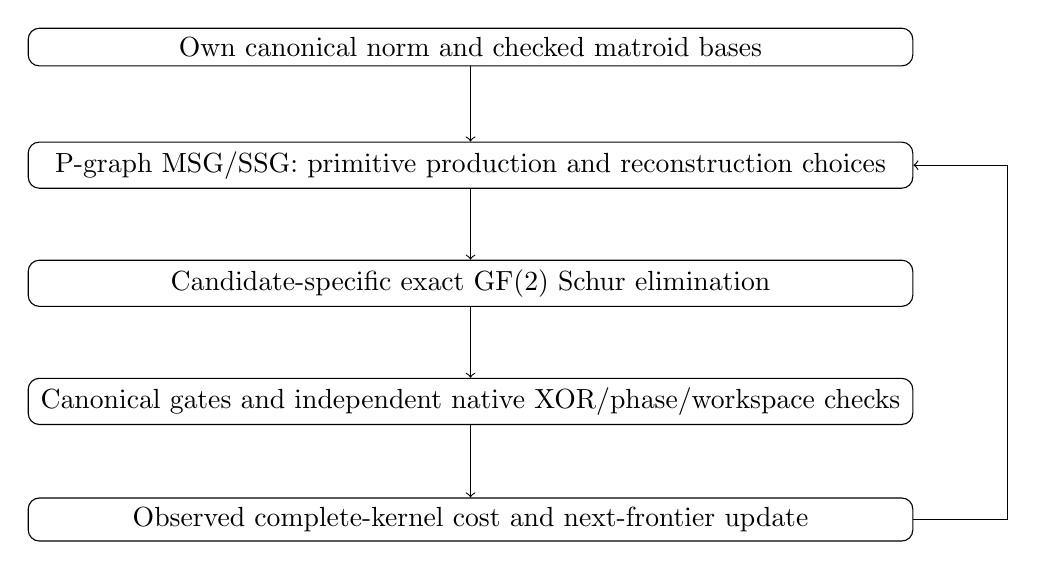
\begin{tikzpicture}[every node/.style={draw,rounded corners,align=center,text width=11cm},node distance=15mm]
\node (a) {Own canonical norm and checked matroid bases};
\node (b) [below of=a] {P-graph MSG/SSG: primitive production and reconstruction choices};
\node (c) [below of=b] {Candidate-specific exact GF(2) Schur elimination};
\node (d) [below of=c] {Canonical gates and independent native XOR/phase/workspace checks};
\node (e) [below of=d] {Observed complete-kernel cost and next-frontier update};
\draw[->] (a)--(b);\draw[->] (b)--(c);\draw[->] (c)--(d);\draw[->] (d)--(e);
\draw[->] (e.east)--++(12mm,0)|-(b.east);
\end{tikzpicture}
\end{center}
\end{document}
